\documentclass{korigamik}

\usepackage{minted}
\usepackage{xcolor}
\usepackage{listings}
\usepackage{algpseudocode}
\usepackage{algorithm}

\title{Data Communications}
\titlelabel{Lab Report}
\bottomnote{Department of Computer Science \& Engineering}
\author{Kushagra Lakhwani}
\rollno{2021UCI8036}
\semester{4th}
\course{CICPC12}
\logoimage{res/NSUT.png}{0.6}{Netaji Subhas University \\ of Technology}
\header{}

\colorlet{mycoolgray}{gray!40}
\lstdefinestyle{output}{
	numbers=none, % where to put the line-numbers
	numberstyle=\tiny, % the size of the fonts that are used for the line-numbers     
	backgroundcolor=\color{darkgray},
	basicstyle=\ttfamily\color{white}\footnotesize,
	captionpos=b, % sets the caption-position to bottom
	breaklines=true, % sets automatic line breaking
	breakatwhitespace=false,
	keywordstyle=\color{white}\bfseries,
}

\begin{document}

\maketitle
\newpage

\center\textbf{\large Abstract}

\begin{justify}
	The practical lab report \textit{``Operating Systems''} is the original and unmodified content submitted by \textit{Kushagra Lakhwani} (Roll No. 2021UCI8036).

	The report is submitted to \textit{Dr. Manoj Kumar} Department of Computer Science and Engineering, NSUT, Delhi, for the partial fulfillment of the requirements of the course \textit{``Operating Systems''} (CICPC09).
\end{justify}

\pagebreak


\thispagestyle{empty}
\tableofcontents
\newpage

\section{Fourier Transform}
\label{sec:fourier transform}

\subsection{Objective}
We plot a Rectangular Pulse Signal $x(t)$ in \textit{Matlab} and explore 
its magnitude and phase spectrum of its Fourier Transform.

\subsection{Theory}

MATLAB is a programming language and environment that is widely used for
scientific computing, numerical analysis, and data visualization. It is designed to
support matrix and vector operations, which are fundamental to many scientific and
engineering applications.

The Fourier Transform of a signal $x(t)$ is defined as
\begin{equation}
	X(\omega) = \int_{-\infty}^{\infty} x(t) e^{-j\omega t} dt
\end{equation}

The Fourier Transform of a rectangular pulse is given by
\begin{equation}
	X(\omega) = \frac{1}{2\pi} \int_{-\infty}^{\infty} \frac{1}{\sqrt{1 - (\omega t)^2}} dt
\end{equation}

The magnitude and phase spectrum of the Fourier Transform of a rectangular pulse is given by
\begin{equation}
	|X(\omega)| = \frac{1}{\pi} \sqrt{\frac{\pi}{2} - \omega^2}
\end{equation}
\begin{equation}
	\angle X(\omega) = \frac{\pi}{2} - \arctan(\omega)
\end{equation}


\subsection{Matlab Code}

\inputminted[fontsize=\footnotesize,autogobble]{matlab}{code/fourier.m}

\subsection{Output}

\begin{figure}[!htb]
	\centering
	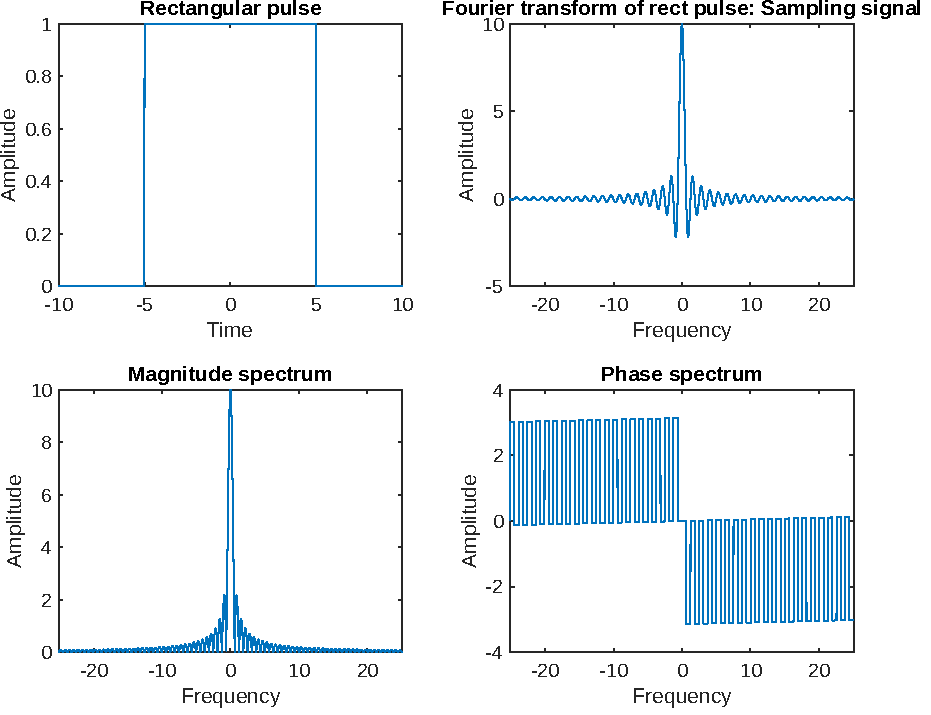
\includegraphics[width=0.7\textwidth]{res/figures/Figure_1.pdf}
	\label{output:fourier transform}
	\caption{Fourier Transform}
\end{figure}
\section{Random Density Function}
\label{sec:random density function}

Using the Gaussian random numbers we find the mean and variance. 

\subsection{Matlab Code}

\inputminted[fontsize=\footnotesize,autogobble]{matlab}{code/density.m}
\subsection{Output}

\begin{figure}[!htb]
	\centering
	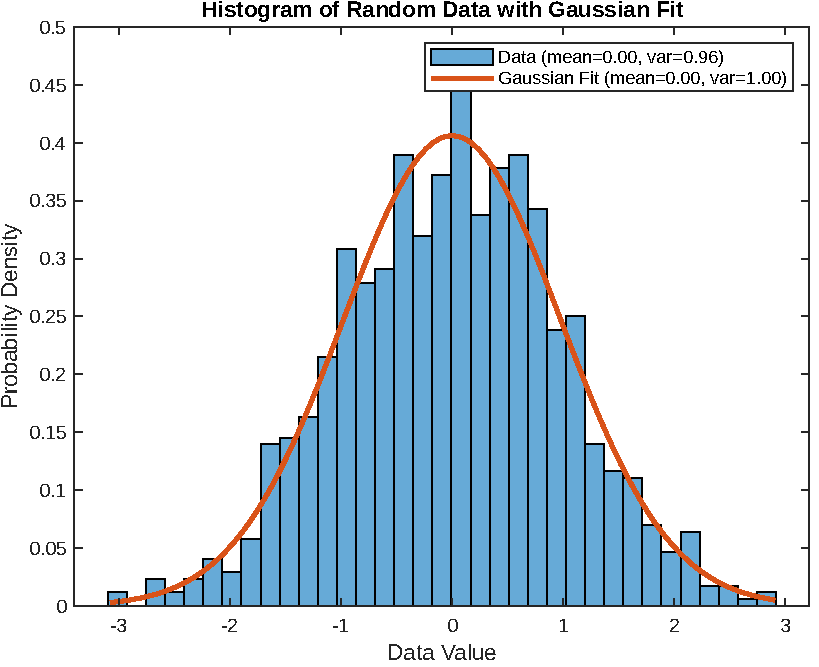
\includegraphics[width=6in]{res/figures/Figure_2.pdf}
	\label{output:gaussian distribution}
	\caption{Gaussian Distribution}
\end{figure}
\section{Quantization: Uniform}
\label{sec:Quantization: Uniform}

Computing the Signal to quantization Noise ratio of Uniform Quantization. 
Plot SNQR vs. Quantization levels.

\subsection{Matlab Code}

\inputminted[fontsize=\footnotesize,autogobble]{matlab}{code/sqnr.m}

\subsection{Output}

\begin{figure}[!htb]
    \centering
    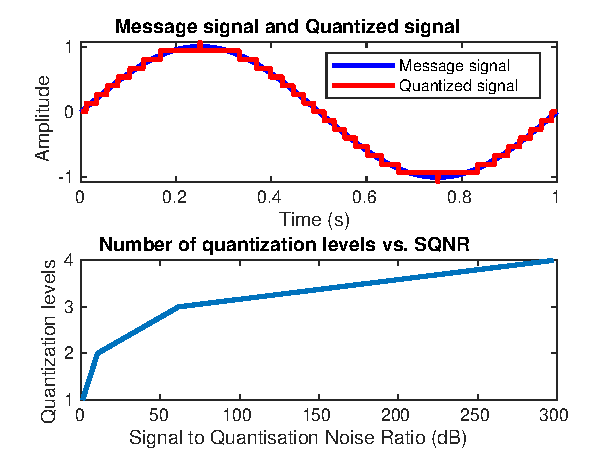
\includegraphics[width=0.8\textwidth]{res/figures/Figure_6.pdf}
    \label{output:SQNR vs quantization}
    \caption{SQNR vs Quantization}
\end{figure}

\section{Quantization: Non-Uniform}
\label{sec:Quantization: Non-Uniform}

Computing SNR of Non-Uniform Quantization and Plot SNR vs. Quantization Levels

\subsection{Matlab Code}

\inputminted[fontsize=\footnotesize,autogobble]{matlab}{code/sqnr2.m}
\subsection{Output}

\begin{figure}[!htb]
    \centering
    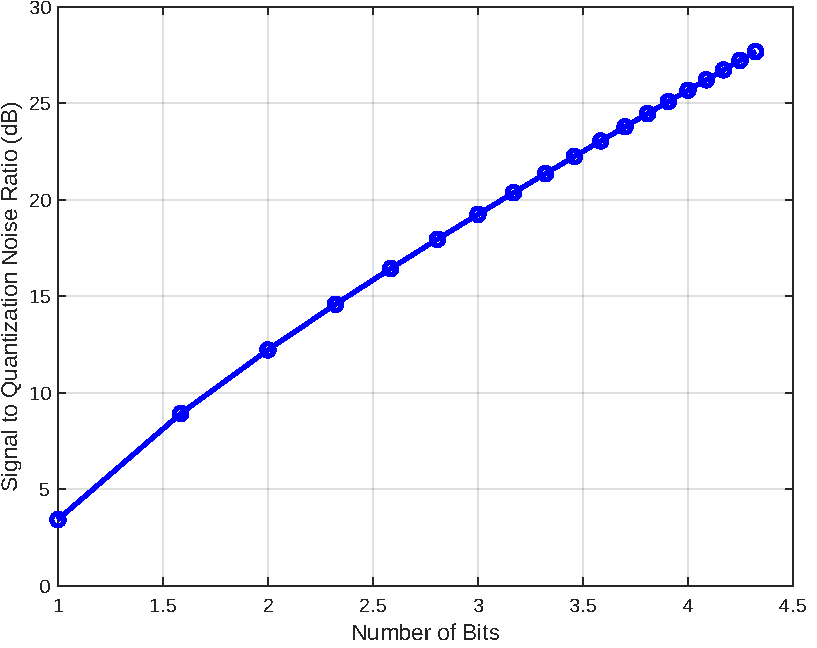
\includegraphics[width=0.7\textwidth]{res/figures/Figure_4.pdf}
    \label{output:SQNR vs quantization 2}
    \caption{SQNR vs Quantization (non-uniform)}
\end{figure}

\end{document}
